\section{Simple Localizer}\label{sec:simple_localizer}
Here we will create a simple localizer taking relative odometry pose measurements and absolute map-based pose measurements as input.
The structure of the localizer is shown in Figure ~\ref{img:simple_localizer}.

\begin{figure}[ht]
    \centering
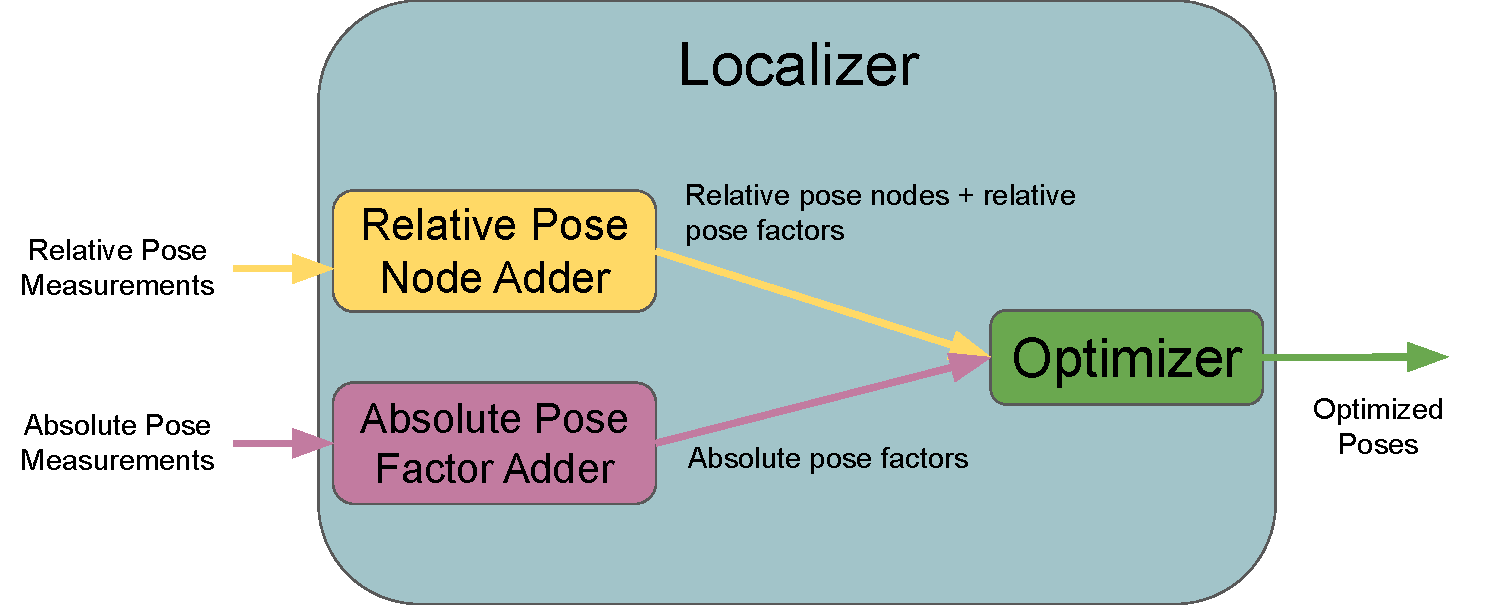
\includegraphics[width=0.9\textwidth]{simple_localizer.pdf}
 \caption{Localizer structure.}
  \label{img:simple_localizer}
\end{figure}
The localizer takes relative and absolute pose measurements and passes these to the node adder and factor adder respectively. 
These are described in more detail below. \par

The graph structure is shown in Figure ~\ref{img:loc_graph}.

\begin{figure}[ht]
    \centering
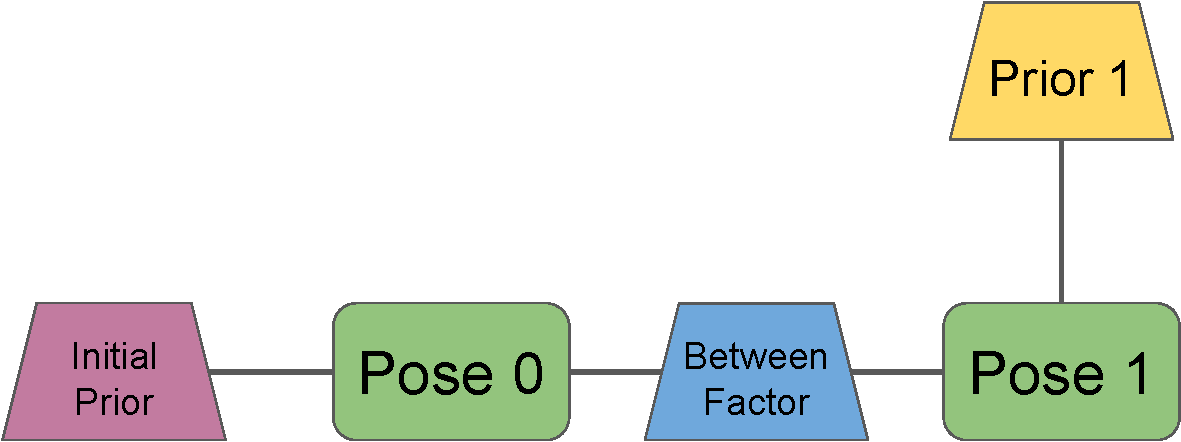
\includegraphics[width=0.9\textwidth]{loc_graph.pdf}
 \caption{Localization graph structure. Optimized pose nodes are connected by pose between factors. An initial prior constrains the first node and absolute measurement priors are added to future nodes.}
  \label{img:loc_graph}
\end{figure}

Pose nodes are optimized at various timestamps. 
An initial pose prior factor is added to the first pose node, while pose between factors connect successive pose nodes.
Absolute pose priors are added using incoming measurements that trigger the creation of new pose nodes and relative factors at the same timestamp.

\subsection{Localizer Sliding Window Graph Optimizer}
We will make the localizer a sliding-window graph optimizer so that old nodes and factors are removed. 
\begin{minted}[]{c++}
#include <localization_measurements/pose_measurement.h>
#include <sliding_window_graph_optimizer/sliding_window_graph_optimizer.h>

#include "absolute_pose_factor_adder.h"
#include "localizer_params.h"
#include "relative_pose_node_adder.h"

class Localizer : public sliding_window_graph_optimizer::
                    SlidingWindowGraphOptimizer {
 public:
  explicit Localizer(const LocalizerParams& params)
      : params_(params) {
    // Register factor and node adders
    AddFactorAdder(factor_adder_);
    AddSlidingWindowNodeAdder(node_adder_);
  }

  void AddRelativePoseMeasurement(
    const localization_measurements::
      TimestampedPoseWithCovariance& measurement) {
    node_adder_->AddMeasurement(measurement);
  }

  void AddAbsolutePoseMeasurement(
    const localization_measurements::
      TimestampedPoseWithCovariance& measurement) {
    factor_adder_->AddMeasurement(measurement);
  }

  const TimestampedNodes<gtsam::Pose3>& timestamped_nodes()
    const {
    return node_adder_->nodes();
  }

 private:
  LocalizerParams params_;

  std::shared_ptr<AbsolutePoseFactorAdder> factor_adder_;
  std::shared_ptr<RelativePoseNodeAdder> node_adder_;
};
\end{minted}
The graph localizer includes both the relative pose node adder and absolute pose factor adder. 

\subsection{Relative Pose Node Adder}
The pose node adder uses timestamped relative pose measurements to create gtsam::Pose3 nodes. 
It relies on the pose node adder model for node and relative factor creation.
\begin{minted}[]{c++}
#include <localization_measurements/timestamped_pose_with_covariance.h>
#include <node_adders/measurement_based_timestamped_node_adder.h>
#include <nodes/timestamped_nodes.h>

#include <gtsam/geometry/Pose3.h>

"relative_pose_node_adder_model.h"

  using RelativePoseNodeAdder =
    MeasurementBasedTimestampedNodeAdder<
      localization_measurements::TimestampedPoseWithCovariance,
      gtsam::Pose3, nodes::TimestampedNodes<gtsam::Pose3>,
      RelativePoseNodeAdderModel>;
\end{minted}
\subsubsection{Pose Measurement}
A timestamped pose with covariance is used to generate values for future node and relative factors.
\subsubsection{Pose Node and TimestampedNodes}
The node type is a gtsam::Pose3 and the timestamped nodes type is a TimestampedNodes object since the node type is a single value.
\subsubsection{Relative Pose Node Adder Model}
\begin{minted}[]{c++}
#include <localization_common/pose_with_covariance_interpolater.h>
#include <localization_measurements/timestamped_pose_with_covariance.h>
#include <node_adders/between_factor_node_adder_model.h>
#include <nodes/timestamped_nodes.h>

#include <gtsam/geometry/Pose3.h>
#include <gtsam/inference/Key.h>

#include <utility>

class RelativePoseNodeAdderModel
    : public BetweenFactorMeasurementBasedTimestampedNodeAdderModel<
        localization_measurements::TimestampedPoseWithCovariance,
        gtsam::Pose3> {
 public:
  using NodesType = nodes::TimestampedNodes<gtsam::Pose3>;
  using Params = TimestampedNodeAdderModelParams;

  explicit PoseNodeAdderModel(const Params& params)
      : Base(params) {}

  gtsam::KeyVector AddNode(
    const localization_common::Time timestamp,
    NodesType& nodes) const final {
    const auto pose = interpolator_.Interpolate(timestamp);
    return nodes.Add(timestamp, pose->pose);
  }

  boost::optional<
    std::pair<gtsam::Pose3, gtsam::SharedNoiseModel>>
  RelativeNodeAndNoise(
    const localization_common::Time timestamp_a,
    const localization_common::Time timestamp_b) const final {
    const auto relative_pose =
      interpolator_.Relative(timestamp_a, timestamp_b);
    const auto relative_pose_noise =
      gtsam::noiseModel::Gaussian::Covariance(
        relative_pose->covariance);
    return std::pair<gtsam::Pose3, gtsam::SharedNoiseModel>(
      relative_pose->pose, relative_pose_noise);
  }

  void AddMeasurement(
    const localization_measurements::
      TimestampedPoseWithCovariance& measurement) {
    interpolator_.Add(measurement.time,
                      measurement.pose_with_covariance);
  }

  void RemoveMeasurements(
    const localization_common::Time oldest_allowed_time) {
    // Keep lower bound so future measurements can be
    // interpolated using it.
    interpolator_.RemoveBelowLowerBoundValues(
      oldest_allowed_time);
  }
  bool CanAddNode(
    const localization_common::Time timestamp) const final {
    return interpolator_.WithinBounds(timestamp);
    ;
  }

 private:
  localization_common::PoseWithCovarianceInterpolater
    interpolator_;
};
\end{minted}
The pose node adder model uses a pose interpolator to generate required relative poses and covariances using input relative pose measurements.
Since the model is a between factor adder model, it inserts gtsam::Pose3 between factors as relative factors.
\subsection{Absolute Pose Factor Adder}
The absolute pose factor adder creates a GTSAM pose prior factor for each absolute pose measurement.
Since each created factor uses a single measurement, the factor adder is a SingleMeasurementBasedFactorAdder.
When adding the prior factor, it uses the relative pose node adder to add a pose node at the same timestamp as the prior factor.
\begin{minted}[]{c++}
#include <factor_adders/absolute_pose_factor_adder_params.h>
#include <factor_adders/single_measurement_based_factor_adder.h>
#include <localization_common/time.h>
#include <localization_measurements/timestamped_pose_with_covariance.h>

class AbsolutePoseFactorAdder
    : public SingleMeasurementBasedFactorAdder<
        localization_measurements::
          TimestampedPoseWithCovariance> {
 public:
  AbsolutePoseFactorAdder(
    const AbsolutePoseFactorAdderParams& params,
    const std::shared_ptr<RelativePoseNodeAdder> node_adder)
      : SingleMeasurementBasedFactorAdder<
          localization_measurements::
            TimestampedPoseWithCovariance>(params),
        params_(params),
        node_adder_(node_adder) {}

 private:
  int AddFactorsForSingleMeasurement(
    const localization_measurements::
      TimestampedPoseWithCovariance& measurement,
    gtsam::NonlinearFactorGraph& factors) final {
    node_adder_->AddNode(measurement.timestamp, factors);
    const auto keys = node_adder_->Keys(measurement.timestamp);
    // First key is pose key
    const auto& pose_key = keys[0];
    const auto pose_noise =
      gtsam::Prior<gtsam::Pose3>::shared_ptr pose_prior_factor(
        new gtsam::Prior<gtsam::Pose3>(
          pose_key, measurement.pose.pose, pose_noise));
    factors.push_back(pose_prior_factor);
  }

  bool CanAddFactor(
    const localization_common::Time time) const final {
    return node_adder_->CanAddNode(time);
  }

  std::shared_ptr<PoseNodeAdderType> node_adder_;
  AbsolutePoseFactorAdderParams params_;
};
\end{minted}
\subsection{Interfacing with Localizer}
Measurements are passed to the node and factor adders at various timestamps. 
Optimization, factor and node creation, and sliding the window occur during the Update() call.
Various helper functions exist for accessing optimized values and covariances from the localizer.
\begin{minted}[]{c++}
#include "localizer.h"

int main() {
  Localizer localizer(LocalizerParams());
  // Add relative and absolute pose measurements at successive
  // timestamps
  for (int i = 0; i < 10; ++i) {
    localizer.AddRelativePoseMeasurement(
      RandomPoseMeasurement(i));
    localizer.AddAbsolutePoseMeasurement(
      RandomPoseMeasurement(i));
  }

  localizer.Update();

  // Access optimized timestamped nodes
  const auto& timestamped_nodes = localizer.timestamped_nodes();
  // Access optimized GTSAM values
  const auto& values = localizer.values();
  // Access GTSAM factors
  const auto& factors = localizer.factors();
  // Compute covariance for a node at timestamp 1
  const auto keys = timestamped_nodes.Keys(1);
  const auto covariance = localizer.Covariance(keys[0]);
}
\end{minted}